% ============================================================================
% Auto-generated from live research-assessment data (regenerate via
% scratchpad/kz-results.mjs). Requires: tikz, xcolor, colortbl, graphicx,
% longtable, booktabs, array. Map border: public Kazakhstan boundary GeoJSON.
% ============================================================================

\section{A Working Demonstration: Kazakhstan's Commercial Research Landscape}
\label{sec:demo}

To show that the system's measurement layer is a functioning instrument rather
than a promise, we applied it to Kazakhstan's research base: every
Kazakhstan-affiliated publication and researcher was scored for commercial,
scientific, and social potential. The results below---a national map, an
institutional ranking, the specific topical fronts on which each institution is
commercially strong, and the leading researchers behind that work---were produced
automatically and are continuously refreshable as the corpus grows. They
correspond to Work Packages~1 and~2.

\begin{figure}[t]
\centering
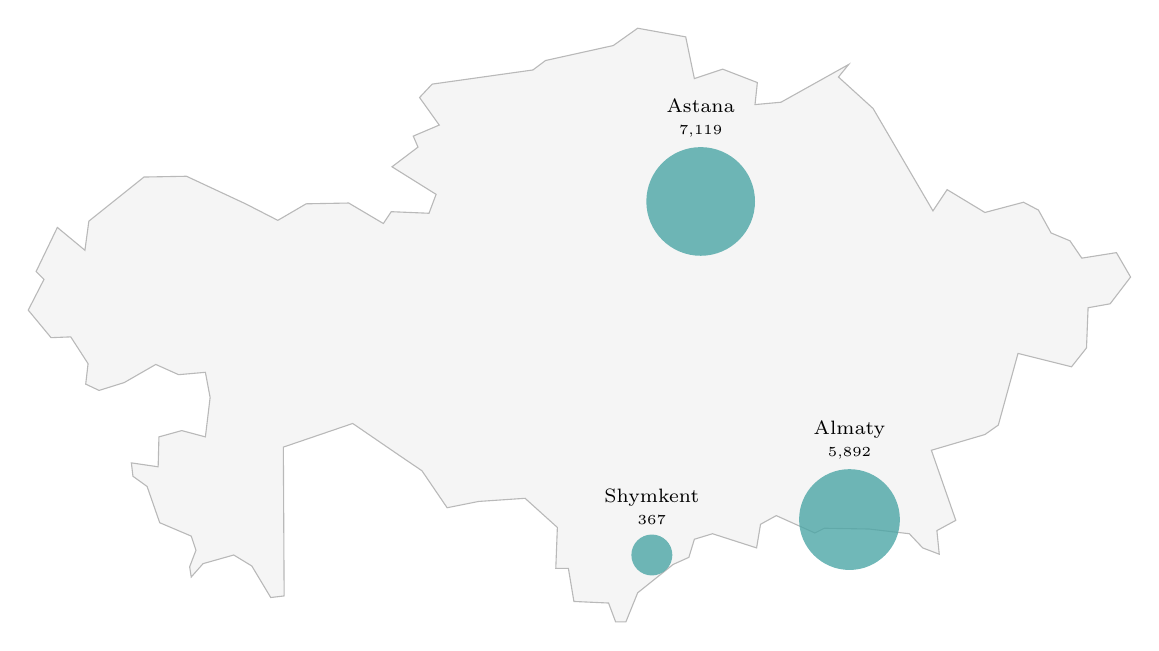
\begin{tikzpicture}[x=1cm,y=1cm]
  \filldraw[fill=gray!8, draw=gray!55, line width=0.4pt] (8.39,0.82) -- (8.19,0.73) -- (7.74,0.37) -- (7.59,0.00) -- (7.46,0.00) -- (7.37,0.24) -- (6.93,0.26) -- (6.86,0.68) -- (6.70,0.68) -- (6.72,1.20) -- (6.31,1.57) -- (5.72,1.53) -- (5.32,1.45) -- (5.00,1.92) -- (4.72,2.11) -- (4.18,2.48) -- (4.12,2.52) -- (3.24,2.22) -- (3.25,0.33) -- (3.08,0.31) -- (2.84,0.71) -- (2.61,0.85) -- (2.22,0.74) -- (2.07,0.57) -- (2.05,0.70) -- (2.13,0.91) -- (2.07,1.09) -- (1.67,1.26) -- (1.51,1.72) -- (1.33,1.85) -- (1.31,2.02) -- (1.65,1.97) -- (1.66,2.35) -- (1.95,2.43) -- (2.25,2.35) -- (2.31,2.85) -- (2.25,3.17) -- (1.91,3.14) -- (1.62,3.27) -- (1.22,3.04) -- (0.90,2.94) -- (0.73,3.02) -- (0.76,3.28) -- (0.54,3.62) -- (0.29,3.61) -- (0.00,3.96) -- (0.20,4.35) -- (0.10,4.45) -- (0.37,5.01) -- (0.72,4.72) -- (0.77,5.09) -- (1.47,5.65) -- (2.01,5.66) -- (2.76,5.31) -- (3.17,5.10) -- (3.53,5.31) -- (4.07,5.32) -- (4.51,5.06) -- (4.61,5.21) -- (5.09,5.19) -- (5.18,5.43) -- (4.62,5.78) -- (4.95,6.03) -- (4.89,6.17) -- (5.22,6.31) -- (4.97,6.66) -- (5.13,6.83) -- (6.41,7.01) -- (6.57,7.13) -- (7.43,7.32) -- (7.74,7.54) -- (8.35,7.43) -- (8.46,6.90) -- (8.82,7.02) -- (9.26,6.85) -- (9.23,6.57) -- (9.56,6.60) -- (10.42,7.08) -- (10.29,6.92) -- (10.73,6.52) -- (11.49,5.22) -- (11.67,5.49) -- (12.15,5.20) -- (12.64,5.33) -- (12.83,5.23) -- (12.99,4.94) -- (13.23,4.84) -- (13.38,4.62) -- (13.82,4.69) -- (14.00,4.38) -- (13.74,4.04) -- (13.46,3.99) -- (13.44,3.48) -- (13.25,3.24) -- (12.57,3.41) -- (12.32,2.50) -- (12.15,2.38) -- (11.47,2.18) -- (11.78,1.29) -- (11.54,1.16) -- (11.57,0.86) -- (11.36,0.94) -- (11.19,1.12) -- (10.68,1.18) -- (10.11,1.19) -- (9.99,1.13) -- (9.50,1.35) -- (9.30,1.24) -- (9.25,0.94) -- (8.69,1.12) -- (8.46,1.05) -- (8.39,0.82) -- cycle;
  \fill[teal!70,opacity=0.8] (8.54,5.34) circle (0.69);
  \node[font=\scriptsize, above=0.69cm, align=center] at (8.54,5.34) {Astana\\{\tiny 7,119}};
  \fill[teal!70,opacity=0.8] (10.43,1.30) circle (0.64);
  \node[font=\scriptsize, above=0.64cm, align=center] at (10.43,1.30) {Almaty\\{\tiny 5,892}};
  \fill[teal!70,opacity=0.8] (7.92,0.85) circle (0.26);
  \node[font=\scriptsize, above=0.26cm, align=center] at (7.92,0.85) {Shymkent\\{\tiny 367}};
\end{tikzpicture}
\caption{Geography of high-commercial-potential research across Kazakhstan. Bubble area is proportional to the number of Kazakhstan-affiliated publications with commercial potential $\geq 0.6$ at each city's institutions. Output concentrates sharply in Astana and Almaty, with Shymkent emerging---a spatial concentration that is itself a finding for regional innovation and talent policy.}
\label{fig:kz-map}
\end{figure}

Figure~\ref{fig:kz-map} locates the nation's commercially promising science;
Table~\ref{tab:kz-rank} ranks the institutions that produce it. Crucially,
Table~\ref{tab:kz-keywords} moves past broad disciplines to the \emph{specific}
research fronts---keyword signatures---on which each institution is strong, the
resolution at which commercialisation decisions are actually made.

\begin{table}[t]
\centering\small
\begin{tabular}{@{}p{7.2cm} l r r@{}}
\toprule
\textbf{Institution} & \textbf{City} & \textbf{High-CP} & \textbf{Mean CP} \\
\midrule
Nazarbayev University & Astana & 5,094 & 99 \\
Al-Farabi Kazakh National University & Almaty & 3,711 & 97 \\
L. N. Gumilyov Eurasian National University & Astana & 2,025 & 93 \\
Satbayev University & Almaty & 1,068 & 91 \\
Kazakh-British Technical University & Almaty & 621 & 82 \\
Kazakh National Medical University & Almaty & 492 & 86 \\
M.Auezov South Kazakhstan State University & Shymkent & 367 & 69 \\
\bottomrule
\end{tabular}
\caption{Kazakhstani institutions ranked by volume of high-commercial-potential research. \textbf{High-CP}: count of Kazakhstan-affiliated publications scoring $\geq 0.6$ for commercial potential. \textbf{Mean CP}: mean commercial-potential score (0--100) of each institution's 100 top-scored outputs.}
\label{tab:kz-rank}
\end{table}

\begin{table}[t]
\centering\small
\begin{tabular}{@{}p{4.6cm} p{10.4cm}@{}}
\toprule
\textbf{Institution} & \textbf{Specific topical strengths (most frequent keywords among its highest commercial-potential work)} \\
\midrule
Nazarbayev University & Fiber Optic Sensors, Distributed Sensing, Biosensors, Haptic Interfaces, Audio-Visual Speech Recognition, Cancer Immunotherapy, Car T Cells \\
\addlinespace
Al-Farabi Kazakh National University & Neural Machine Translation, Two-Dimensional Materials, Machine Translation, Multilingual Neural Machine Translation, Language Modeling, Self-Assembled Monolayers, Translation \\
\addlinespace
L. N. Gumilyov Eurasian National University & Membrane Fouling, Nanocrystal Synthesis, Wastewater Treatment, Immunity, Deep Learning, Sustainable Water Treatment, Membrane Technology \\
\addlinespace
Satbayev University & Polymeric Gels, Controlled Polymerization, Adsorption, Hydrogels, Hydrogen Production, Graphene, Surfactants \\
\addlinespace
Kazakh-British Technical University & Named Entity Recognition, Information Retrieval, Color Psychology, Aesthetic Intelligence, Ionic Liquids, Detection, Language Modeling \\
\addlinespace
Kazakh National Medical University & Asthma, Aging, Mesenchymal Stem Cells, Nk Cell Therapy, Nk Cell Development, Car T Cells, Nk Cell Recognition \\
\addlinespace
M.Auezov South Kazakhstan State University & Nanoencapsulation, Dyeing, Integro-Differential Equations, Plant Growth, Wastewater Treatment, Inverse Problems, Inverse Scattering Theory \\
\bottomrule
\end{tabular}
\caption{The concrete research fronts, not broad disciplines, where each institution's commercially promising work concentrates. These keyword signatures reveal genuine specialisation: photonic and fiber-optic sensing and cell therapy at Nazarbayev; batteries, graphene, and hydrogen at Satbayev; machine translation and two-dimensional materials at Al-Farabi; membranes and water treatment at Gumilyov; stem-cell and NK/CAR-T therapy at the medical university.}
\label{tab:kz-keywords}
\end{table}

Finally, a commercialisation strategy is executed by people. Table~\ref{tab:kz-researchers}
identifies the leading Kazakhstan-based researchers by the commercial potential
of their work, with the topics they work on---the human capital the strategy must
engage, retain, and connect to industry and to the diaspora.

\begin{table}[t]
\centering\small
\begin{tabular}{@{}p{3.1cm} p{3.5cm} p{6.2cm} r r@{}}
\toprule
\textbf{Researcher} & \textbf{Institution} & \textbf{Topics} & \textbf{Pubs} & \textbf{CP} \\
\midrule
Vesselin N. Paunov & Nazarbayev University & Pickering Emulsions, Microemulsions, Nanoparticles, Droplet Formation & 137 & 90 \\
\addlinespace
Daniele Tosi & Nazarbayev University & Fiber Optic Sensors, Refractive Index Sensor, Distributed Sensing, Long-Period Gratings & 96 & 88 \\
\addlinespace
Yuliya Semenova & Nazarbayev University & Fiber Optic Sensors, Refractive Index Sensor, Sensor Technology, Whispering Gallery Mode & 120 & 88 \\
\addlinespace
Zhumabay Bakenov & Nazarbayev University & Battery Materials, Nanostructured Cathodes, Nanostructured Anodes, Lithium-Sulfur Batteries & 122 & 88 \\
\addlinespace
Woojin Lee & Nazarbayev University & Reductive Dechlorination, Nano Zero-Valent Iron, Metastatic Pancreatic Cancer, High-Efficiency Solar Cells & 546 & 86 \\
\addlinespace
Kyunghwan Oh & Nazarbayev University & Microstructured Optical Fibers, Fiber Lasers, Nonlinear Optics, Fiber Optic Sensors & 100 & 86 \\
\addlinespace
Thierry Djenizian & Al-Farabi Kazakh National University & Anode Materials, Nanostructured Anodes, Electrode Materials, Battery Materials & 87 & 85 \\
\addlinespace
Michael Hippler & Institute of Plant Biology and Biotechnology & Photosynthetic Acclimation, Photosystem II, Light-Harvesting, Photocycle Dynamics & 98 & 84 \\
\addlinespace
Ferdinand Molnár & Nazarbayev University & Vitamin D, Epigenetic Reprogramming, Tumor Evolution, Cancer Epigenetics & 68 & 84 \\
\addlinespace
Danil Bukhvalov & Satbayev University & Graphene, Metal-Organic Frameworks, Single-Molecule Magnets, Graphene Oxide & 197 & 84 \\
\bottomrule
\end{tabular}
\caption{The people behind the science: leading Kazakhstan-based researchers by the commercial potential of their work (of 2,369 indexed Kazakhstan-affiliated researchers with sustained output). \textbf{CP}: mean commercial potential (0--100). This is the human capital a commercialisation strategy must engage, retain, and connect.}
\label{tab:kz-researchers}
\end{table}
